%%%%%%%%%%%%%%%%%%%%%%%%%%%%%%%%%%%%%%%%%
% Beamer Presentation
% LaTeX Template
% Version 1.0 (10/11/12)
%
% This template has been downloaded from:
% http://www.LaTeXTemplates.com
%
% License:
% CC BY-NC-SA 3.0 (http://creativecommons.org/licenses/by-nc-sa/3.0/)
%
%%%%%%%%%%%%%%%%%%%%%%%%%%%%%%%%%%%%%%%%%

%----------------------------------------------------------------------------------------
%	PACKAGES AND THEMES
%----------------------------------------------------------------------------------------

\documentclass{beamer}

\mode<presentation> {

% The Beamer class comes with a number of default slide themes
% which change the colors and layouts of slides. Below this is a list
% of all the themes, uncomment each in turn to see what they look like.

%\usetheme{default}
%\usetheme{AnnArbor}
%\usetheme{Antibes}
%\usetheme{Bergen}
%\usetheme{Berkeley}
%\usetheme{Berlin}
%\usetheme{Boadilla}
%\usetheme{CambridgeUS}
%\usetheme{Copenhagen}
%\usetheme{Darmstadt}
%\usetheme{Dresden}
%\usetheme{Frankfurt}
%\usetheme{Goettingen}
%\usetheme{Hannover}
%\usetheme{Ilmenau}
%\usetheme{JuanLesPins}
%\usetheme{Luebeck}
\usetheme{Madrid}
%\usetheme{Malmoe}
%\usetheme{Marburg}
%\usetheme{Montpellier}
%\usetheme{PaloAlto}
%\usetheme{Pittsburgh}
%\usetheme{Rochester}
%\usetheme{Singapore}
%\usetheme{Szeged}
%\usetheme{Warsaw}

% As well as themes, the Beamer class has a number of color themes
% for any slide theme. Uncomment each of these in turn to see how it
% changes the colors of your current slide theme.

%\usecolortheme{albatross}
%\usecolortheme{beaver}
%\usecolortheme{beetle}
%\usecolortheme{crane}
%\usecolortheme{dolphin}
%\usecolortheme{dove}
%\usecolortheme{fly}
%\usecolortheme{lily}
%\usecolortheme{orchid}
%\usecolortheme{rose}
%\usecolortheme{seagull}
%\usecolortheme{seahorse}
%\usecolortheme{whale}
%\usecolortheme{wolverine}

%\setbeamertemplate{footline} % To remove the footer line in all slides uncomment this line
%\setbeamertemplate{footline}[page number] % To replace the footer line in all slides with a simple slide count uncomment this line

%\setbeamertemplate{navigation symbols}{} % To remove the navigation symbols from the bottom of all slides uncomment this line
}
\DeclareMathOperator*{\argmin}{arg\,min}
\newcommand{\argminD}{\arg\!\min}
%\usepackage[utf8]{inputenc}
%\usepackage[normalem]{ulem}
\usepackage{subcaption}
\usepackage[font=scriptsize]{caption}
\usepackage{multicol}
\usepackage{scalerel}
\usepackage{amsmath}
\usepackage{graphicx} % Allows including images
\graphicspath{{./images/}}
\usepackage{booktabs} % Allows the use of \toprule, \midrule and \bottomrule in tables

%----------------------------------------------------------------------------------------
%	TITLE PAGE
%----------------------------------------------------------------------------------------

\title[M-estimator]{Channel Estimation Techniques for Multicarrier OFDM 5G Wireless Communication Systems} % The short title appears at the bottom of every slide, the full title is only on the title page

\author{Jeevan} % Your name
\institute[IITH] % Your institution as it will appear on the bottom of every slide, may be shorthand to save space
{
IITH\\ % Your institution for the title page

CS20BTECH11047
%\medskip
%\textit{john@smith.com} % Your email address
}
\date{} % Date, can be changed to a custom date

\begin{document}








\begin{frame}
\titlepage % Print the title page as the first slide
\end{frame}


%-------------------------------------------------------------------------------------------------------------------------------
\begin{frame}{}

\begin{block}{Authors}
\begin{itemize}
    \item Tipparti Anil Kumar, CMR Hyderabad
    \item Lokam Anjaneyulu , NIT Warangal
\end{itemize}
\end{block}

\begin{block}{Abstract}
\begin{itemize}
    \item We will discuss about channel estimation techniques in multicarrier 
orthogonal frequency-division-multiplexing (OFDM) 5G 
wireless communication systems in Rayleigh and Rician 
channels.
    \item Proposed M-estimator based channel estimation 
technique in comparison with classical least squares (LS) and 
linear minimum mean-squared error (LMMSE) estimation is 
studied and analyzed.
\item We will compare the proposed technique over LS and LMMSE through simulations .
\end{itemize}


\end{block}
    
\end{frame}
%-----------------------------------------------------------------------------------------------------------------------------

\begin{frame}{System Model}
\begin{itemize}
    \item OFDM is one of the efficient modulation formats used in present 5G wireless communication systems.
\end{itemize}
\begin{figure}
    \centering
    \includegraphics[scale =0.2]{images/OFDM system.png}
    \caption{Block diagram of OFDM system with FFT}
    \label{fig:OFDM}
\end{figure}
    
\end{frame}
%-------------------------------------------------------------------------
\begin{frame}{System Model}
The received signal (at the receiver) may be described by\\
\begin{align}
    \mathbf{Y=HX+W}
\end{align}
where
\begin{align}
    \mathbf{H}=\left[ H[0], H[1],....., H[N-1]  \right]^{T}\\
    \mathbf{W}=\left[ W[0], W[1],....., W[N-1]  \right]^{T}\\
    \mathbf{X}=\begin{bmatrix}
    X[0] & 0 & \cdots & 0\\
    0    & X[1] &  &  \vdots\\
    \vdots &  & \ddots & 0\\
    0 & \cdots &0 & X(N-1)
    \end{bmatrix}
\end{align}
    
\end{frame}
%------------------------------------------------------------


%------------------------------------------------

\begin{frame}{M-Estimator}
consider a  signal model
\begin{align}
    r_{j}=\sum_{k=1}^{K} s_{j}^{k} \theta _{k} + n_{j}  , \quad j=1,2,....,N
    \end{align}
     or in matrix notation
    \begin{align}
    \underline{r}=\underline{S} \underline{\theta} + \underline{n}
\end{align}
where
\begin{align}
    \underline{S}\triangleq \left[ \underline{s_{1}}, \underline{s_{2}},    \cdots    \underline{s_{K}}\right]\\
    \underline{\theta } \triangleq \left[ \theta _{1},  \theta _{2}, \cdots  \theta _{K} \right]^{T}
\end{align}
\end{frame}

%------------------------------------------------

\begin{frame}
\frametitle{M-Estimator}
Huber proposed to minimize a sum of a less rapidly increasing function  $\rho$ of the residuals
\begin{align}
\label{eq:1}
    \underline{\hat{\theta}}=\argminD_{\theta \in \mathcal{R}^{K}} \sum^{N}_{j=1} \rho \left( r_{j} - \sum^{K} _{k=1} s^{k}_{j} \theta_{k} \right)
\end{align}
suppose that $\rho$ has a derivative $\psi=\rho'$; then , the solution to ($\ref{eq:1}$) satisfies the equation
 \begin{align}
 \label{eq:2}
\sum_{j=1}^{N}\psi \left( r_{j} - \sum _{l=1} ^{K} s^{l}_{j} \theta_{l}  \right) s^{k}_{j} =0, \quad k=1,2,.........,K
\end{align}
or in vector form
\begin{align}
    S^{T}\psi\left(\underline{r}-\underline{S}\underline{\theta}\right)= \underline{0}_{K}\\
\text{where} \quad      \psi(\underline{x}) \triangleq \left[ \psi(x_{1}) ,....,\psi(x_{K}) \right]^{T} \text{for any } \underline{x} \in \mathcal{R}^{K}
\end{align}
\end{frame}

%------------------------------------------------

\begin{frame}
\frametitle{M-Estimator}
Assume that the penalty function $\rho(x)$ in ($\ref{eq:1}$) has a bounded second-order derivative i.e., $|\rho''(x)|=|\psi ' (x)| \leq \mu$ for some $\mu > 0$.
Then ($\ref{eq:2}$) can be solved iteratively by the following modified residual method . Let $\underline{\theta}^{t}$ be the estimated at the $t$th step;then it is updated according to 
\begin{align}
    \underline{z}^{t} \triangleq \psi \left(\underline{r}-\underline{S} \underline{\theta}^{t} \right)\\
    \underline{\theta}^{t+1} = \underline{\theta}^{t} + \dfrac{1}{\mu} \left(\underline{S}^{T} \underline{S}\right)^{-1} \underline{S}^{T} \underline{z}^{t}
\end{align}
where $\mu$ is a step-size parameter .$\left( \mu = \dfrac{1}{N} \sum_{j=1}^{N} \psi ' \left( r_{j} - \sum^{K} _{k=1} s^{k}_{j} \theta_{k} ^{t} \right) \right)$\\
For initial estimate $\underline{\theta^{0}}$, we can take 
\begin{align}
    \underline{\theta}^{0} = \dfrac{1}{\mu} \left( \underline{S}^{T} \underline {S} \right)^{-1} \underline{S}^{T} \underline{r}.
\end{align}
The iteration is stopped if $\lVert  \underline{\theta}^{t} - \underline{\theta}^{t-1} \rVert \leq \epsilon $   for some small number $\epsilon$ .
\end{frame}

%------------------------------------------------
%------------------------------------------------
\begin{frame}
\frametitle{Proposed M-Estimator}
Penalty, influence and weight functions of the proposed M-estimator for channel estimation in 5G multicarrier wireless 
communications in Rayleigh and Rician fading channels are given by
\begin{align}
    \rho_{\scaleto{PROPOSED}{3.5pt}}(x)= \begin{cases}   
    \dfrac{x^2}{2} &  \lvert x \rvert \leq a \\
    a^2-a\lvert x \rvert &  a <\lvert x \rvert \leq b\\
    \dfrac{-ab}{2} \exp\left(1- \dfrac{x^2}{b^2} \right) + d &  \lvert x \rvert>b
    \end{cases}
\end{align}
\begin{align}
    \psi_{\scaleto{PROPOSED}{3.5pt}}(x)= \begin{cases}   
    x &  \lvert x \rvert \leq a\\
    asgn(x)  &  a <\lvert x \rvert \leq b\\
    \dfrac{a}{b}x \exp\left(1- \dfrac{x^2}{b^2} \right) &  \lvert x \rvert>b
    \end{cases}
\end{align}

\end{frame}

%------------------------------------------------

\begin{frame}
\frametitle{Proposed M-Estimator}
\begin{align}
    \mathnormal{w}_{\scaleto{PROPOSED}{3.5pt}}(x)= \begin{cases}   
    1 &  \lvert x \rvert \leq a\\
    \dfrac{asgn(x)}{x} &  a <\lvert x \rvert \leq b\\
    \dfrac{a}{b} \exp\left(1- \dfrac{x^2}{b^2} \right) &  \lvert x \rvert>b
    \end{cases}
\end{align}
where $a$ and $b$ are any constants and $x$ is any data. From an influence function, robustness measures are derived and $a(=kv^2)$ and $b(=2kv^2)$ are selected (where $k$ is any constant).\\
where $\rho(x)$ is penalty function,  $\psi(x)=\dfrac{d\rho(x)}{dx}$ is the influence function and $w(x)=\dfrac {\psi(x)}{x}$ is the weight function. 
\end{frame}

%------------------------------------------------

\begin{frame}{Proposed M-Estimator}
\begin{multicols}{3}
\begin{figure}
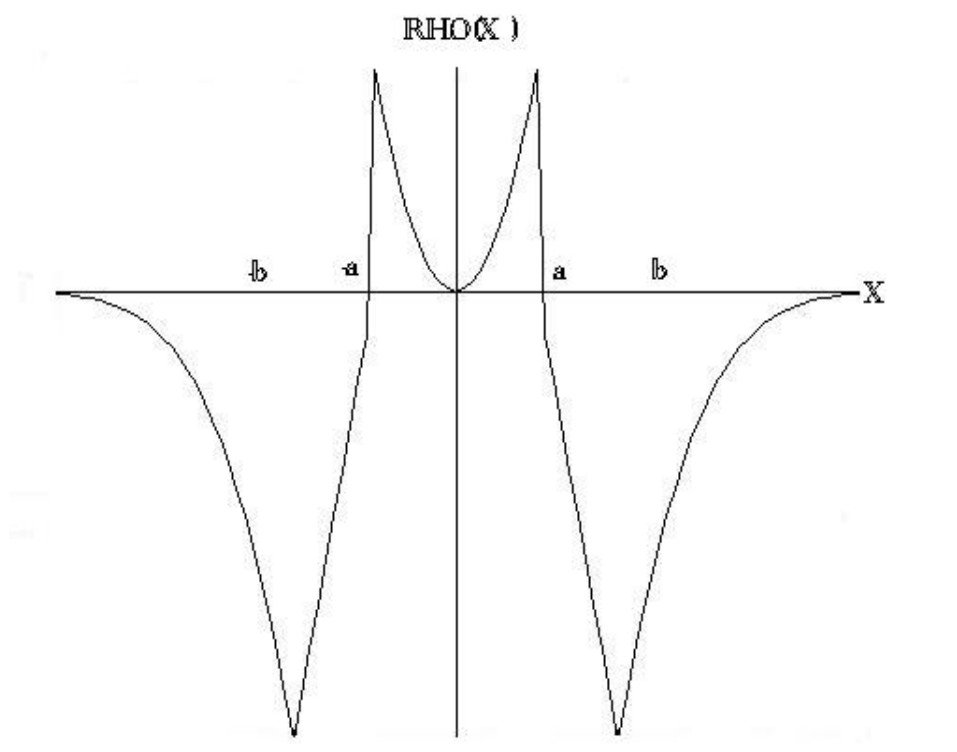
\includegraphics[scale=0.15]{images/rho.png}
\caption{  Proposed M-estimator penalty function.}
\label{fig:rho}
\end{figure}
\begin{figure}
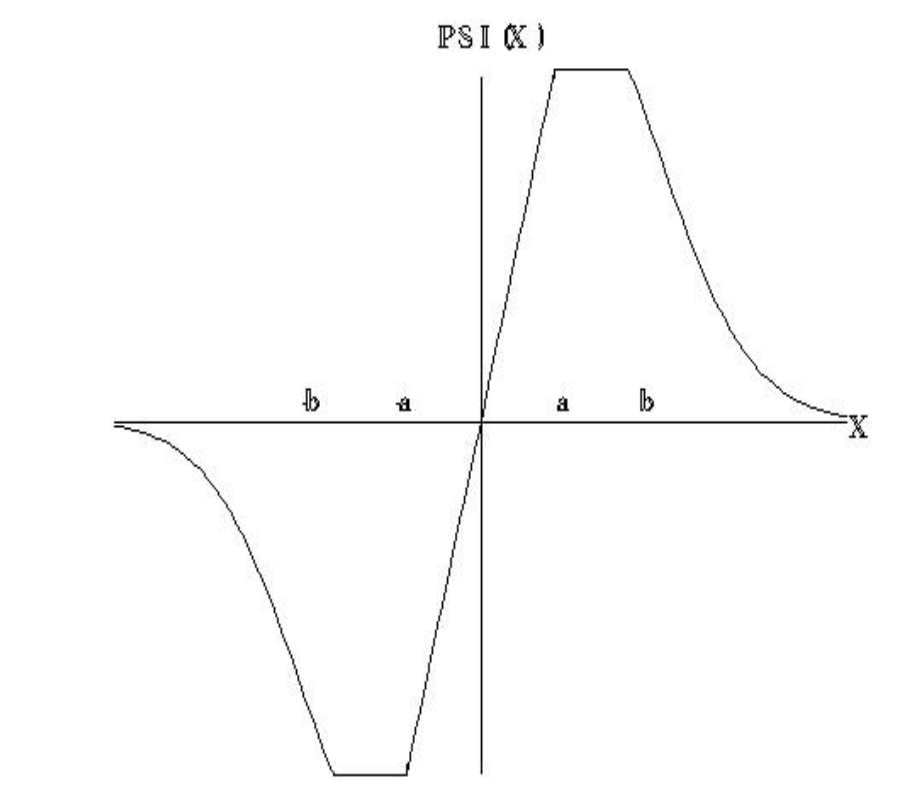
\includegraphics[scale=0.15]{images/psi.png}
\caption{ Proposed M-estimator influence function}
\label{fig:psi}
\end{figure}
\begin{figure}
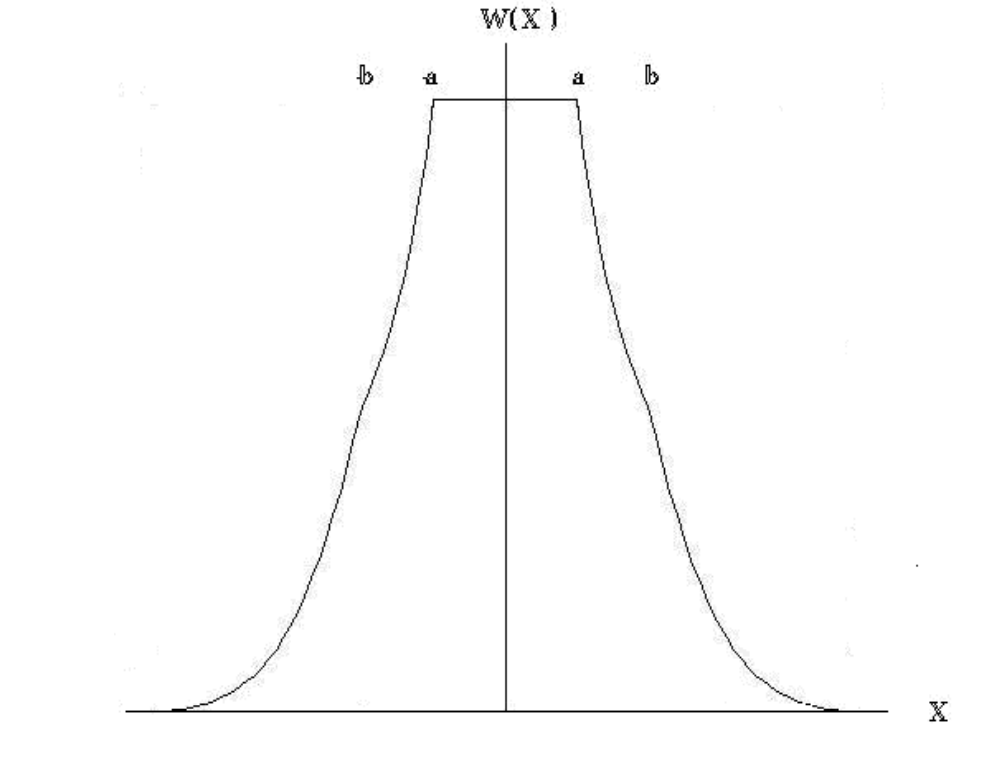
\includegraphics[scale=0.15]{images/weight.png}
\caption{Proposed M-estimator weight function}
\label{fig:w}
\end{figure}
\end{multicols}
\end{frame}

%------------------------------------------------

\begin{frame}
\frametitle{Channel Estimation}
\begin{block}{LS channel estimation}
\begin{align}
    \hat{H}_{LS} = \left( X^{H} X \right)^{-1} X^{H}Y =X^{-1}Y
\end{align}
where estimate of $H$ is $\hat{H}$ and $X^{H}$ is the Hermitian matrix of $X$ 
\end{block}
\begin{block}{MMSE channel estimation}
\begin{align}
    \hat{H}_{MMSE}= R_{HH} \left[ R_{HH} + \left( X X^{H}\right)^{-1} W \mathnormal{v}^{2} \right]^{-1} \hat{H}_{LS}
\end{align}
where $R_{HH}$ is the matrix form of auto-covariance of $X$ and
   $\mathnormal{v}^{2}$ is variance of noise vector.
\end{block}
\end{frame}

%------------------------------------------------



%------------------------------------------------

\begin{frame}
\frametitle{Channel Estimation}
\begin{block}{proposed estimation}
Proposed technique estimates channel parameters for 5G 
multicarrier wireless communications in Rayleigh and Rician 
fading channels using
\begin{align}
    H^{t+1}=H^{t} + \dfrac{1}{\mu} \left( X^{H}X\right)^{-1} X^{H} \psi \left( Y-HX \right)
\end{align}
for some $\mu > 0$ where $H^{0}=\dfrac{1}{\mu} \hat{H}_{LS}$

\end{block}
\end{frame}

%------------------------------------------------

\begin{frame}{SIMULATION RESULTS}
 In this simulation , the comparison shows the performance gains achieved by the proposed technique over LS and MMSE estimation in 
multicarrier OFDM 5G wireless communication systems
\begin{figure}
\begin{subfigure}{.5\textwidth}
  \centering
  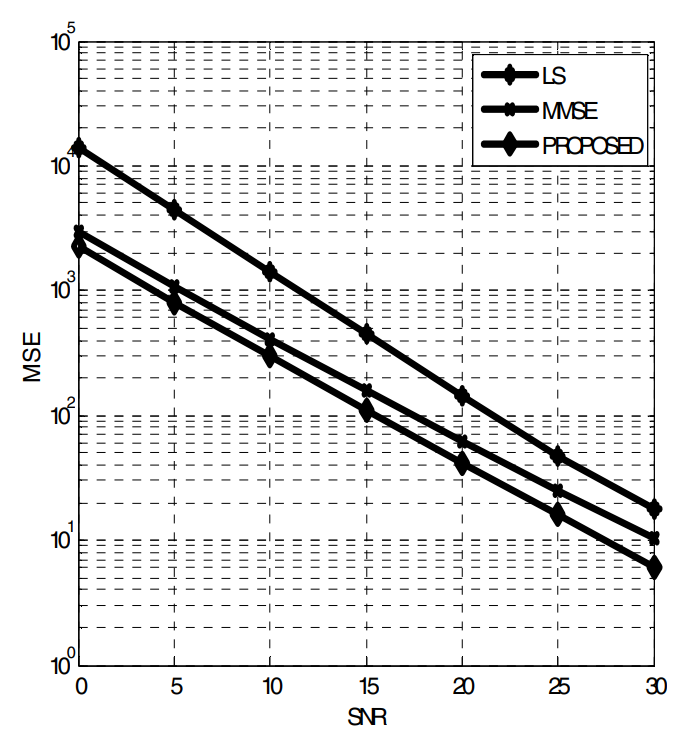
\includegraphics[width=.8\linewidth]{images/Rayleigh.png}
  \caption{}
  \label{fig:Rayleigh}
\end{subfigure}%
\begin{subfigure}{.5\textwidth}
  \centering
  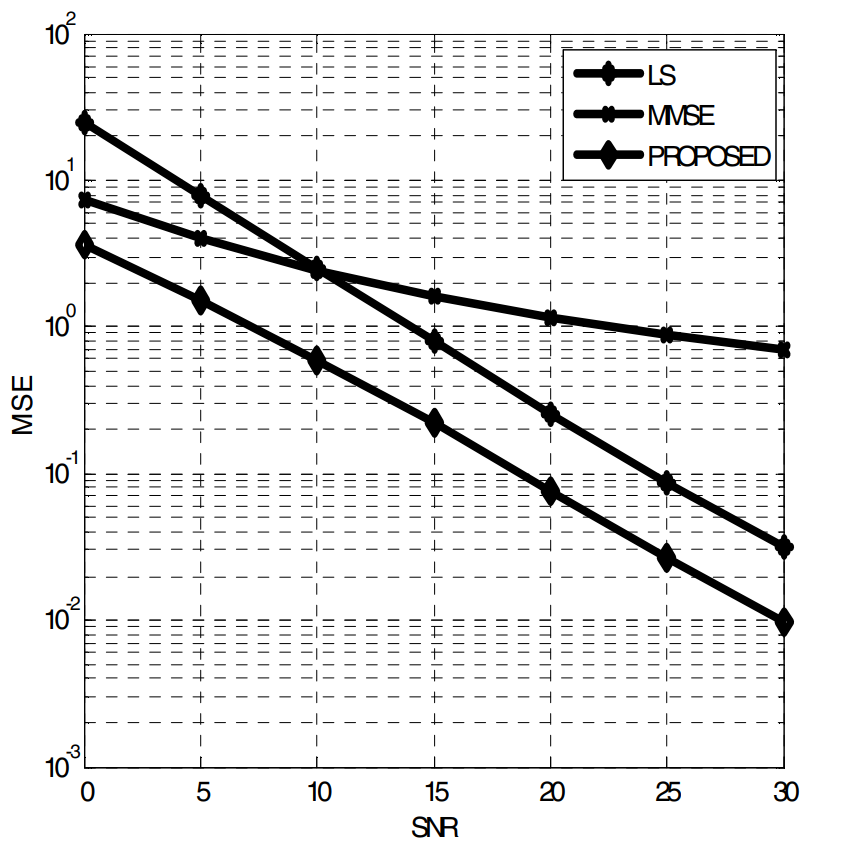
\includegraphics[width=.8\linewidth]{images/Rician.png}
  \caption{}
  \label{fig:Rician}
\end{subfigure}
\caption{{\tiny MSE vs. SNR Performance of LS, MMSE and Proposed channel estimators in (a) Rayleigh and (b) Rician fading channels}}
\label{fig:fig}
\end{figure}
\end{frame}

%----------------------------------------------------------------------------------------
\begin{frame}{CONCLUSION}

\begin{itemize}
    \item M-estimator based channel estimation technique for 5G 
multicarrier OFDM wireless communication systems in 
Rayleigh and Rician fading channels is analyzed in this paper.
    \item Observations from simulation results imply that 
the proposed M-estimator based channel estimation technique 
for 5G multicarrier OFDM wireless communication systems 
offers better performance than LS and MMSE techniques in 
Rayleigh and Rician fading channels. 
\end{itemize}
\end{frame}
\end{document}